\documentclass[tikz]{standalone}
\usepackage{amsmath}
\usetikzlibrary{arrows.meta,
                bending,
                calc, chains,
                quotes,
                positioning,
                shapes.geometric,
                decorations.pathreplacing,
                calligraphy,
                automata}

\definecolor{pantone2727}{RGB}{48,127,226}

\begin{document}

    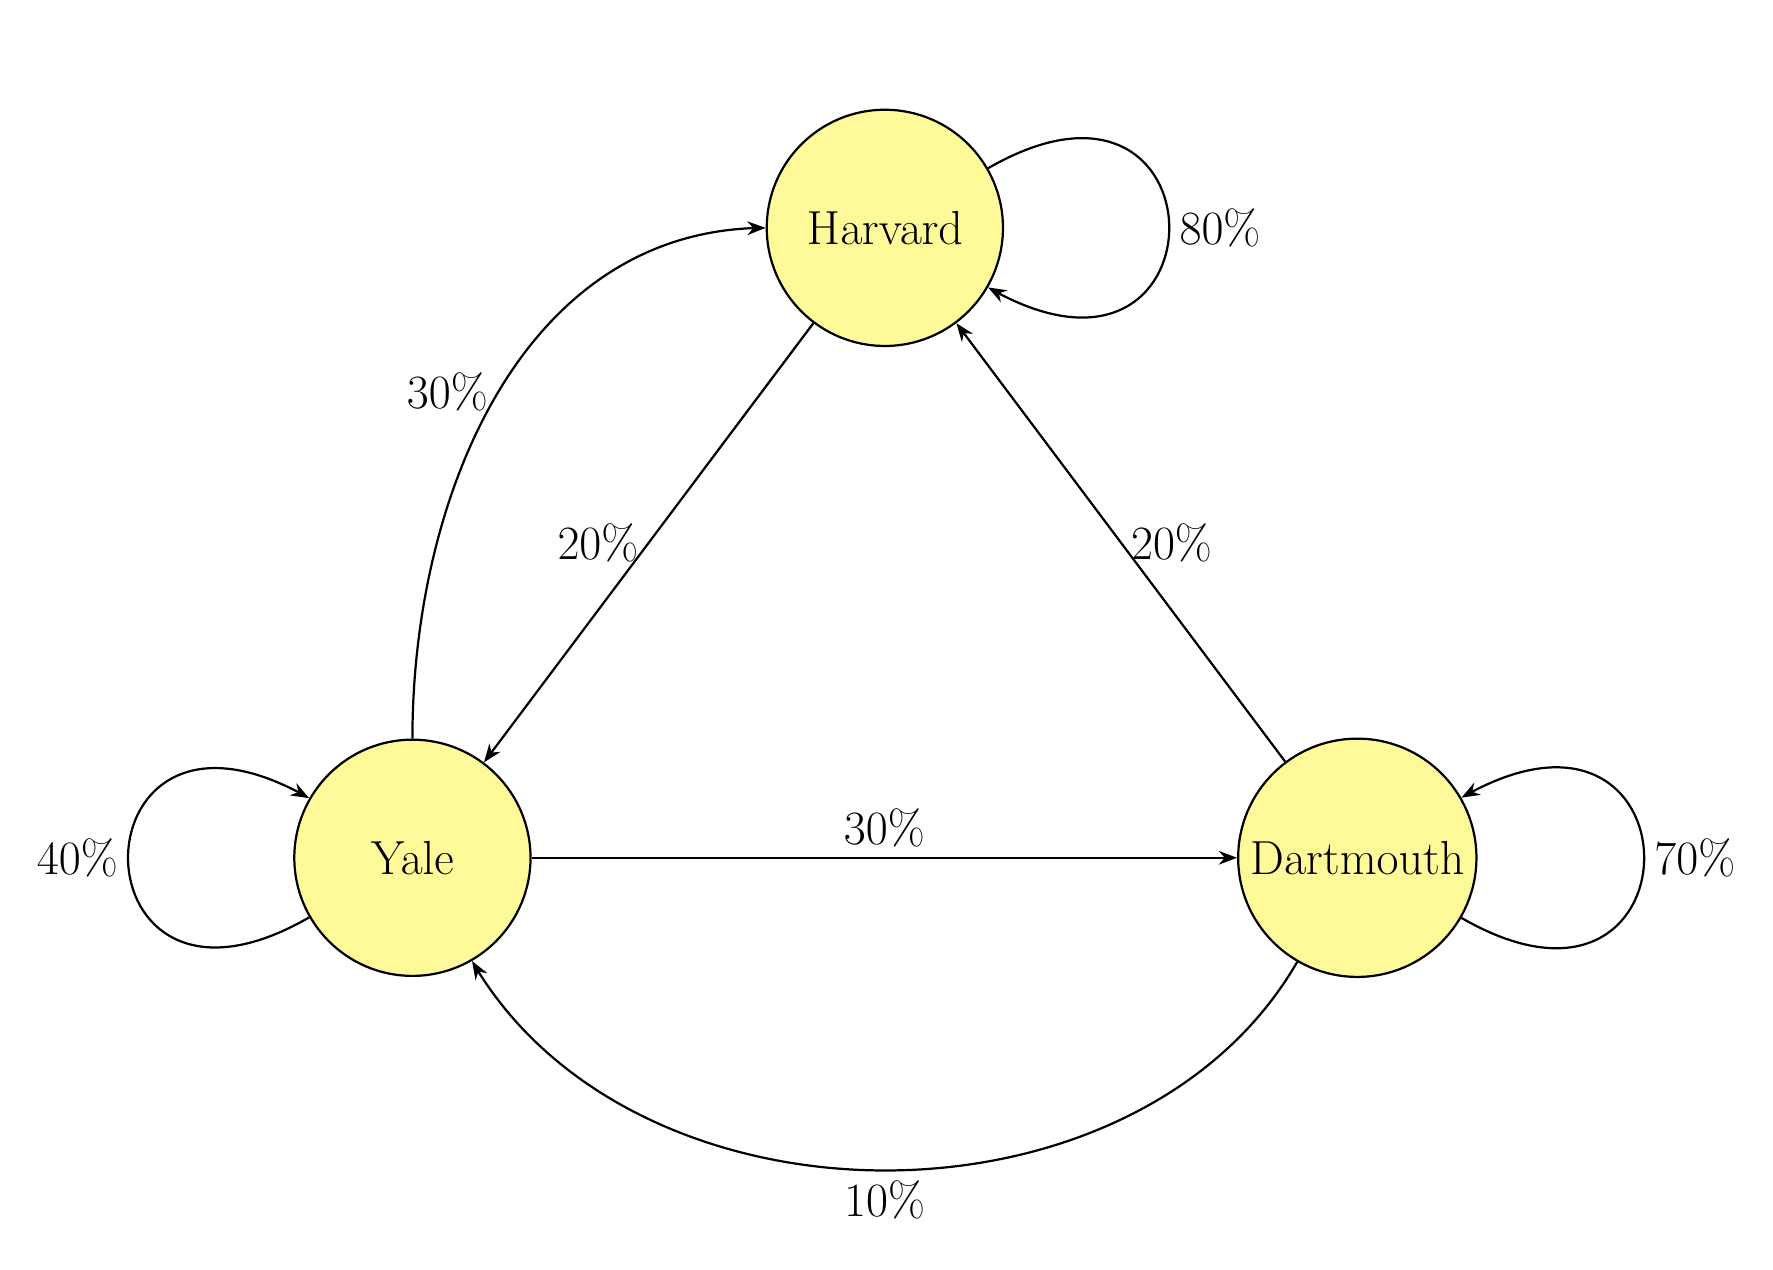
\begin{tikzpicture}[
        node distance=2cm,
        startstop/.style={rectangle, rounded corners, minimum width=3cm, minimum height=1cm,text centered, draw=black, fill=red!30},
        process/.style={rectangle, minimum width=3cm, minimum height=1cm, text centered, draw=black, fill=orange!30},
        io/.style={trapezium, trapezium left angle=70, trapezium right angle=110, minimum width=3cm, minimum height=1cm, text centered, draw=black, fill=blue!30},
        decision/.style={diamond, minimum width=3cm, minimum height=1cm, text centered, text width=3cm, draw=black, fill=green!30},
        end/.style={rectangle, minimum width=3cm, minimum height=1cm, text centered, rounded corners, draw=black, fill=green!30},
        connector/.style={circle, minimum size=3cm, text centered, draw=black, thick, fill=yellow!40}
        ]

        \node (node1)  [connector]                                            {\LARGE Harvard};
        \node (node2)  [connector, below of=node1, xshift=-6cm, yshift=-6cm]  {\LARGE Yale};
        \node (node3)  [connector, below of=node1, xshift=6cm, yshift=-6cm]   {\LARGE Dartmouth};

        \draw [arrows=-Stealth, thick] (node1)  -- node[anchor=east]               {\LARGE $20\%$}           (node2);
        \draw [arrows=-Stealth, thick] (node2)  -- node[anchor=west]    [above]    {\LARGE $30\%$}       (node3);
        \draw [arrows=-Stealth, thick] (node3)  -- node[anchor=north]   [right]    {\LARGE $20\%$}  (node1);

        \draw [->, -Stealth, thick] (node1) to[in=330, out=30, looseness=6] node[midway,right] {\LARGE ${80\%}$} (node1);
        \draw [->, -Stealth, thick] (node2) to[in=150, out=210, looseness=6] node[midway,left] {\LARGE $40\%$} (node2);
        \draw [->, -Stealth, thick] (node2) to[in=180, out=90, looseness=1] node[midway, left]  {\LARGE $30\%$} (node1);
        \draw [->, -Stealth, thick] (node3) to[in=30, out=330, looseness=6] node[midway, right] {\LARGE $70\%$} (node3);
        \draw [->, -Stealth, thick] (node3) to[in=300, out=240,looseness=1] node[midway, below] {\LARGE $10\%$} (node2);

    \end{tikzpicture}


\end{document} 